\documentclass[border=1pt]{standalone}
\usepackage{tikz}

\begin{document}
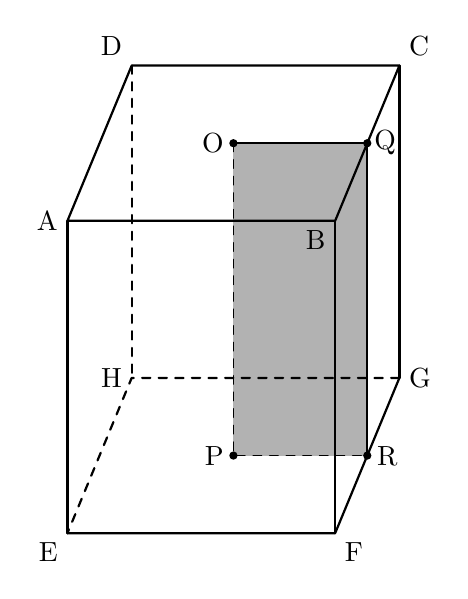
\begin{tikzpicture}[x={(0.24cm, 0.58cm)}, y={(1cm, 0cm)}, z={(0cm, 1cm)},     
    line join=round, line cap=round]   
                
    % パラメータの定義
    \pgfmathsetmacro{\X}{3.4} % 奥行き
    \pgfmathsetmacro{\Y}{\X} % 横幅
    \pgfmathsetmacro{\Z}{\X/6*7} % 高さ
       
    % 頂点の座標定義 (x, y, z)
    \coordinate (E) at (0,0,0); 
    \coordinate (F) at (0,\Y,0); 
    \coordinate (G) at (\X,\Y,0);
    \coordinate (H) at (\X,0,0);
    \coordinate (A) at (0,0,\Z);
    \coordinate (B) at (0,\Y,\Z);
    \coordinate (C) at (\X,\Y,\Z);
    \coordinate (D) at (\X,0,\Z);
    
    % 中点などの定義
    \coordinate (Q) at (\X/2,\Y,\Z);
    \coordinate (R) at (\X/2,\Y,0);
    \coordinate (O) at (\X/2,\Y/2,\Z);
    \coordinate (P) at (\X/2,\Y/2,0);

    % 網掛け
    \fill[black!30] (O) -- (Q) -- (R) -- (P) -- cycle;

    % 線の描画（奥の隠れる線）
    \draw [thick, dashed] (G) -- (H) -- (E);
    \draw [thick, dashed] (D) -- (H);
    \draw [semithick, dashed] (O) -- (P) -- (R);

    % 線の描画（見える実線）
    \draw [thick] (A) -- (B) -- (C) -- (D) -- cycle;
    \draw [thick] (E) -- (F) -- (G);
    \draw [thick] (A) -- (E);
    \draw [thick] (B) -- (F);
    \draw [thick] (C) -- (G);
    \draw [semithick] (O) -- (Q) -- (R);

    % 頂点とラベル
    \foreach \p in {O,P,Q,R} \fill (\p) circle (1.5pt);
    \node[left] at (A) {A};
    \node[below left] at (B) {B};
    \node[above right] at (C) {C};
    \node[above left] at (D) {D};
    \node[below left] at (E) {E};
    \node[below right] at (F) {F};
    \node[right] at (G) {G};
    \node[left] at (H) {H};
    \node[left] at (O) {O};
    \node[left] at (P) {P};
    \node[right, xshift=-1pt] at (Q) {Q};
    \node[right] at (R) {R};
    
\end{tikzpicture}
\end{document}